\section{Cifrari perfetti}
Sono cifrari che offrono una sicurezza incondizionata, con certezza assoluta di fronte a qualsiasi potenza di calcolo.
Con un sistema perfetto anche un attacco a forza bruta non può romperlo.

Si paga un caro prezzo nella loro implementazione, infatti si usano solo per pochi ambiti,
per la crittografia comune si preferisce avere una sicurezza computazionale scommettendo su $P \neq NP$.

Questo concetto è stato formalizzato da Shannon (nel 1949) informalmente un
cifrario è perfetto se la sicurezza è garantita qualunque sia l'informazione carpita dal canale.
Abbiamo lo spazio dei messaggi $MSG$ e lo spazio dei crittogrammi $CRITTO$.

Abbiamo poi le variabili aleatorie $M \in MSG$ che descrive il comportamento del mittente e $C \in CRITTO$ che descrive il processo di comunicazione sul canale.

\begin{itemize}
    \item P(M=m) : probabilità che il mittente voglia spedire il messaggio m
    \item P(M=m $ \mid $ C=c) : probabilità condizionata (a posteriori) che il messaggio inviato sia m posto che sul canale transita $C \in CRITTO$
\end{itemize}

Si suppone che il crittoanalista conosca tutto il sistema tranne la chiave. Conosce:
\begin{itemize}
    \item distribuzione di probabilità con cui il mittente invia un messaggio
    \item conosce il cifrario
    \item conosce lo spazio delle chiavi K
\end{itemize}

\emph{Un cifrario è perfetto se $\forall m \in MSG$, $\forall c \in CRITTO$ vale:}
$$ P(M=m  \mid  C=c) = P(M=m) $$

Cioè: la conoscenza di C non ci permette di inferire nulla sul messaggio.

Es: supponiamo: 
$$P(M=\bar{m}) = p > 0, 0 < p < 1$$
$$\exists \bar{m}, \bar{c} : P(M=\bar{m} \mid C=\bar{c}) = 1$$
si ha quindi che se sul canale passa $\bar{c}$ il messaggio è sicuramente $\bar{m}$ quindi aumenta la nostra conoscenza sul sistema. Questo sistema non è perfetto!

Es: supponiamo:
$$\exists \bar{c} : P(M=\bar{m} \mid C=\bar{c}) = 0$$
ci permette di dire che se non passa $\bar{c}$ non è stato spedito il messaggio m, anche qui la nostra conoscenza aumenta. Questo sistema non è perfetto!

In un cifrario perfetto la conoscenza complessiva del crittoanalista non cambia dopo che è stato osservato un crittogramma in transito: m e c sono del tutto scorrelati, c appare essere una sequenza casuale.

\subsection{Th di Shannon}
\emph{In un cifrario perfetto il numero delle chiavi deve essere maggiore o uguale al numero dei messaggi possibili}
\subsubsection{Dimostrazione}
$$N_m = \#\{m \in MSG : P(M=m)>0\}$$
$$N_k = \#\{\text{insieme delle chiavi}\}$$
Supponiamo per assurdo che $N_k < N_m$, presi quindi gli spazi si ha questa situazione:

\begin{figure}[H]
  \centering
  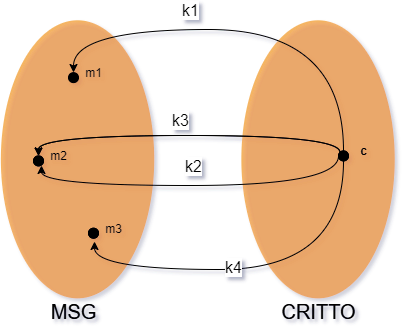
\includegraphics[width = 250pt]{Shannon_proof.png}
\end{figure}

Per i crittogrammi $c : P(C=c) > 0$ possono corrispondere $s$ messaggi, cioè tutti i messaggi che ottengo decriptando $c$ con tutte le chiavi possibili. Si ha necessariamente che $S \leq N_k$ supponendo che chiavi diverse vadano in messaggi diversi si ottiene $S = N_k$ ma magari più chiavi decifrano il messaggio allo stesso modo quindi $S < N_k$. In generale sarà vero che $S \leq N_k$ quindi unendo:
$$ S \leq N_k < N_m \xrightarrow{} S < N_m $$
quindi il numero dei messaggi che possono corrispondere a c è < dei messaggi possibili, quindi deve esistere un $m \in MSG$, $P(M=m) > 0$ tale che:
$$ P(M=m \mid C=c) = 0 $$
(decifrando $c$ esisterà un $m$ che sicuramente non è il messaggio) inferisco della conoscenza, quindi contraddico il cifrario perfetto.

Ne deriva quindi che $N_m \leq N_k$. Per usare un cifrario perfetto mi serve quindi una chiave lunghissima!

\subsection{One-Time Pad}
E' un cifrario precedente Shannon, è simile ad un Vigenère con chiave lunga quanto il messaggio ma su un alfabeto binario. Nasce nel 1917 da Mauborge Vernam. Come alfabeto si usa \{0, 1\}, MSG, CRITTO, KEY sono sequenze binarie e l'algoritmo di cifratura è noto a tutti ed è lo XOR (somma modulo 2):

Supponiamo quindi $m, k \in \{0, 1\}^{n}, n > 0$:
$$ c = C(m, k) = m \oplus k $$
$$ m = D(c, k) = c \oplus k$$

Infatti: $m = c \oplus k = m \oplus k \oplus k = m \oplus 0 = m$

NB: \emph{la chiave deve essere NON riutilizzabile}, se così non fosse si avrebbero problemi:
$$ c_1 = m_1 \oplus k $$
$$ c_2 = m_2 \oplus k $$
$$ c_1 \oplus c_2 = m_1 \oplus k \oplus m_2 \oplus k = m_1 \oplus m_2 $$
non ottengo la chiave, ma se ottengo degli zeri in alcune posizioni, so che lì i due messaggi in chiari sono uguali, quindi ottengo conoscenza sulla chiave/messaggio.

NB: l'unica informazione ottenibile dal one-time-pad è la lunghezza del messaggio

\subsubsection{Teorema sul one-time pad}
Se:
\begin{itemize}
    \item tutti i messaggi hanno lunghezza $n$, se più corti li paddo, se più lunghi li divido in blocchi
    \item tutte le sequenze di $n$ bit hanno probabilità maggiore di zero di essere inviate (tutte le sequenze di bit sono messaggi)
    \item usare una chiave scelta perfettamente a caso per ogni messaggio
\end{itemize}
allora: \emph{one-time pad è perfetto e minimale} (usa un numero minimo di chiavi)

\subsubsection{Dimostrazione perfettezza}
$$ \forall m \in MSG, \forall c \in CRITTO $$
$$ P(M=m \mid C=c) = P(M=m) $$

Si ricordi che:
$$ P(M=m \mid C=c) \triangleq \frac{P(M=m\text{ e }C=c)}{P(C=c)} $$
stimiamo il numeratore: per le proprietà dello XOR fissato $m$ esiste una sola chiave che mi produce $c$ perché chiavi diverse producono crittogrammi diversi:
$$ \nexists k \in KEY: m \oplus k = c $$
quindi la probabilità di ottenere $c$ da $m$ è pari alla probabilità di scegliere casualmente $k$: $\frac{1}{2^n}$
quindi $\forall c \in CRITTO$ $P(C=c)=\frac{1}{2^n}$
nessuna dipendenza dal messaggio quindi sono eventi indipendenti: \{M=m\}, \{C=c\} indipendenti, quindi:
$$ P(C=c\text{ e }M=m) = P(M=m) \cdot P(C=c) $$
tornando alla definizione di perfetto possiamo sostituire:
$$
    P(M=m \mid C=c) = \frac{P(M=m\text{ e }C=c)}{P(C=c)} = \frac{P(M=m) \cdot \cancel{P(C=c)}}{\cancel{P(C=c)}}
$$
siamo arrivati alla definizione di perfetto!

\subsubsection{Dimostrazione minimale}
Da Shannon vale che $N_k \geq N_m$ ma nel one-time pad su lunghezza
$n$ ho $N_k = N_m= N_{CRITTO} = 2^n$.
Anche le chiavi sono sequenze di bit e ne uso il numero minore possibile.

\subsubsection{Osservazioni}
Rimuoviamo l'ipotesi che tutte le sequenze di $n$ bit siano messaggi possibili:
in inglese i messaggi significativi sono solo $\alpha^{n}$ con $\alpha = 1.1 \xrightarrow{} \alpha^n << 2^n$.

Proviamo quindi a ridurre la grandezza della chiave:
$N_m = \alpha^n$ dato che $N_k \geq N_m = \alpha^n$.

La chiave sarà una sequenza di $t$ bit tale che:
$$ t: 2^t \geq \alpha^n \xrightarrow t \geq log_2\alpha^n = n \cdot log_2\alpha \xrightarrow t \geq 0.12 \cdot n$$
Posso quindi usare chiavi molto più corte: $\approx 10\%$ di $n$.

Come fare? Genero i $t$ bit randomicamente e li estendo in maniera deterministica su $n$ bit.
Dobbiamo però metterci al riparo dall'attacco forza bruta: è fondamentale che coppie diverse di
$(m, k)$ producano lo stesso crittogramma. Per far ciò il $\#(m, k)$ deve essere di molto maggiore di $\#CRITTO$:
$$ \alpha^n \cdot 2^t >> 2^n \xrightarrow{} t >> 0.88n$$
In definitiva ci serve $t >> 88\%n$ quindi non si ha una grande compressione della chiave.